\documentclass[a4paper,10pt]{report}
\usepackage[T1]{fontenc}
\usepackage[table]{xcolor}
\usepackage{titlesec}
\usepackage{graphicx}
\usepackage[inkscapepath=../assets/svg]{svg}
\usepackage{amsmath}
\usepackage{amsthm}
\usepackage{mathtools}
\usepackage{fancyvrb}
\usepackage[english]{babel}
\usepackage{csquotes}
\usepackage{verbatim}
\usepackage{hyperref}
\hypersetup{
   colorlinks=true,
   linkcolor=blue,
   urlcolor=cyan
}
\usepackage{tikz}
\usepackage{amssymb}
\usepackage[sc]{mathpazo}
\linespread{1.05}
\usepackage{microtype}
\usepackage{breqn}
\usepackage{caption}
\usepackage{subcaption}
\usepackage[
   backend=bibtex,%
   bibencoding=utf8,%
   language=english,%
   style=numeric-comp,%
   sorting=nyt,%
   maxbibnames=10,%
   natbib=true%
]{biblatex}
\addbibresource{references.bib}
\usepackage{siunitx}
\usepackage{booktabs}
\usepackage{longtable}
\usepackage{geometry}
\usepackage{multirow}
\graphicspath{ {../assets/img/} }

\newgeometry{hmargin={30mm,30mm}}

% Set TOC depth and sections numbering
\setcounter{tocdepth}{3}
\setcounter{secnumdepth}{3}

% Remove chapters head and reduce spacing
\titleformat{\chapter}[hang]{\Large\bfseries}{\thechapter \hspace{2ex}}{0pt}{\Large}
\titlespacing{\chapter}{0cm}{0cm}{0.5cm}
\usepackage[parfill]{parskip}

% Make quotes italic
\renewcommand{\mkbegdispquote}[2]{\itshape}

% Change texttt line breaks
\renewcommand{\texttt}[1]{%
  \begingroup
  \ttfamily
  \begingroup\lccode`~=`.\lowercase{\endgroup\def~}{.\discretionary{}{}{}}%
  \catcode`/=\active\catcode`[=\active\catcode`.=\active
  \scantokens{#1\noexpand}%
  \endgroup
}
\usepackage{amsmath}
\newcommand{\argmin}{\mathop{\mathrm{argmin}}}  

\begin{document}
\frenchspacing

% First page
\title{
  {{\large{\textsc{Alma Mater Studiorum $\cdot$ University of Bologna}}}}
  \rule{\textwidth}{0.4pt}\vspace{3mm}
  \small{Statistical and Mathematical Methods for Artificial Intelligence}

  \large{\textbf{Optimization via Gradient Descent and Stochastic Gradient Descent}}
}

\author{Lorenzo Cellini (\href{mailto:lorenzo.cellini3@studio.unibo.it}{lorenzo.cellini3@studio.unibo.it})}
\date{\today}
\maketitle
\newpage
\tableofcontents
\setcounter{tocdepth}{1}
%\listoffigures
%\listoftables
\newpage


\chapter{Summary}\label{chap:introduction}
Mathematical optimization is the selection of a best element, with regard to some criterion, from some set of available alternatives.
In the simplest case, an optimization problem consists of maximizing or minimizing a real function by systematically choosing input values, from within an allowed set, and computing the value of the function.
More generally, optimization includes finding "best available" values of some objective function given a defined domain (or input), including a variety of different types of objective functions and different types of domains.

Depending on the function and on the real problem, optimization could mean both finding the local/global minimum or finding the local/global maximum, but for historical reasons, the accepted convention is to always talk about minimization and so, when facing a maximization problem, the first step is to change the sign of the function in order to transform it into a minimization one.
However the two approaches are completely equivalent and also procedures to solve them are the same. 
The reason why minimization is the most common approach is related to the idea to minimize an error function when making a numerical approximation.

In this exercise two optimization technique have been explored: Gradient Descent (GD) and Stochastic Gradient Descent (SGD).
Both of them are iterative methods for finding local minimum for differentiable functions, being the second a stochastic approximation of the first one.

This laboratory session consists of two distinct exercises: in the first one Gradient Descent is applied to four different functions and performances are compared for different algorithm parameters;
in the second one Stochastic Gradient Descent is applied to the least square loss function in order to approximate the transformation matrix that map a random generated dataset to the true output vector.

\chapter{Background theory}\label{chap:background}
\section{GD}
An optimization problem can be formulated as: given a function $f:\mathbb{R}^n\rightarrow \mathbb{R}$, with $f\in C^1$ compute the element $x^*$ such that
\begin{equation}
  x^*=\argmin_{x\in \mathbb{R}^n} f(x)
\end{equation}
Such an $x^*$ is a local minimum if, given $\epsilon>0$
\begin{equation}
  \forall x\in \mathbb{R}^n: ||x-x^*||\leq\epsilon \Rightarrow f(x^*)\leq f(x)
\end{equation}

Gradient Descent and Stochastic Gradient Descent are two techniques employed to solve such a problem.
The idea is to compute the gradient of the function in an initial point, move against gradient direction (that points where the function increases) with a predefined step length and repeat until convergence is reached.
Convergence here means that the increasing in the goodness of the solution is less than a certain treshold, being one of the algorithm parameters.

Gradient Descent iteration can be represented as: given an initial point $x_0 \in \mathbb{R}^n$ and a positive step length $\alpha_k$, in each iteration compute
\begin{equation}
  x_{k+1}=x_k - \alpha_k\nabla f(x_k)
\end{equation}

The algorithm ends when it reaches the maximum number of iteration or when the following convergence condition is satisfied:
\begin{equation}
  \begin{gathered}
  ||\nabla f(x_k)||_2 < tol_f||\nabla f(x_0)||_2 \\ \vee \\ ||x_k-x_{k-1}||_2 < tol_x \\ \vee \\ k=k_{max}
\end{gathered}
\label{eq:convergence}
\end{equation}
being $tol_f=1e-5$ and $tol_x=1e-4$ two algorithm parameters.

Sometimes using a fixed step length is not a good practice because the algorithm could end up jumping between the "sides" around the minimum without reaching it.
In order to avoid this behaviour, there exist different techniques that update step length value during computation. Among them there is \emph{backtracking} that can be formulated as:
\begin{equation}
  f(x_k - \alpha_k \nabla f(x_k)) > f(x_k) - c  \alpha_k ||\nabla f(x_k)||^2 \Rightarrow \alpha_{k+1} = \tau \alpha_k
\end{equation}
where $\alpha$ is the step length, $\tau$ a parameter that control the decreasing of $\alpha$ and c a parameter that decides when to update $\alpha$.
Here $c=0.8$ and $\tau=0.25$.
\newpage
\section{SGD}
Usually in machine learning it is not practical to implement standard gradient descent, for example when the dataset to evaluate gradients on is big.
SGD aims to solve this issue by computing, at each iteration, an approximation of the true gradient by evaluating function's derivatives over a subset of samples called batch.
Being all the theory the same, what changes is that, at each iteration, the algorithm does not follow the shortest path toward the minimum but an irregular one close to the it.

A classical machine learning problem can be formulated as before, with the only difference being that now the function to be minimized depends also on the dataset $f(\vec{w},\mathbb{D})$, where $\vec{w}$ is the weights vector.
The problem can be rewritten as finding $\vec{w}^*$ such that
\begin{equation}
  \vec{w}^* = \argmin_{\vec{w}} L(\vec{w},\mathbb{D}) = \argmin_{\vec{w}} \sum_{i=1}^{N} l(\vec{w},x^{(i)},y^{(i)})
\end{equation}
where $L$ is the \emph{loss function} and the summation is carried over the entire dataset $\mathbb{D}$.

Because the goal is to optimize with respect to $\vec{w}$, the training iteration becomes:
\begin{equation}
  \vec{w}_{k+1} = \vec{w}_k - \alpha_k \sum_{i=1}^N \nabla l(\vec{w},x^{(i)},y^{(i)})
\end{equation}


\chapter{Exercise 1 - Gradient Descent}\label{chap:gd}
In the first exercise it is required to implement GD for four different functions and experiment with different hyperparameters. In the following sections the four experiments are reported.
\section{Function \#1}
Optimize function $f:\mathbb{R}^2 \rightarrow \mathbb{R}$ such that
\begin{equation}
  f(x_1,x_2)=(x_1-3)^2+(x_2-1)^2
\end{equation}
where the true optimum is $x^*=(3,1)^T$.

In order to apply GD, the derivative of $f$ has to be computed first. So
\begin{equation}
  \nabla f(x_1,x_2)= [2(x_1-3),2(x_2-1)]
\end{equation}

Graphs in \ref{fig:1} and \ref{fig:1c} show the value of the gradient $\nabla f(\vec{x})$ and the distance between $\vec{x}_{true}$ and $\vec{x}_k$ for each iteration and for different values of $\alpha$.
\begin{figure}[!htb]
  \minipage{0.5\textwidth}
    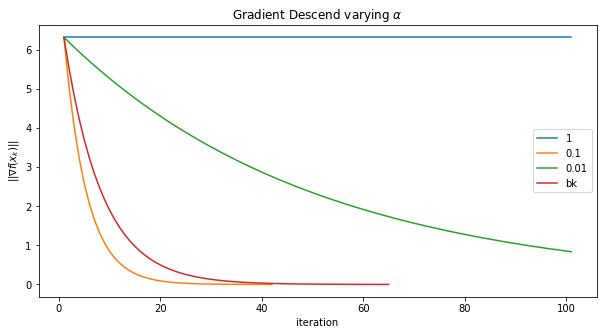
\includegraphics[width=\linewidth]{1_a.png}
  \endminipage\hfill
  \minipage{0.5\textwidth}
    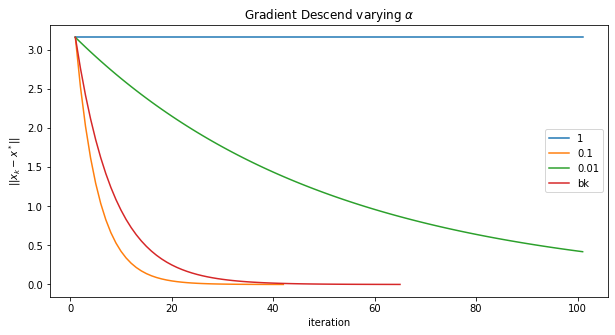
\includegraphics[width=\linewidth]{1_k.png}
  \endminipage\hfill
  \caption{Gradient Descent applied to first function.}
  \label{fig:1}
\end{figure}
\begin{figure}[!htb]
  \center
  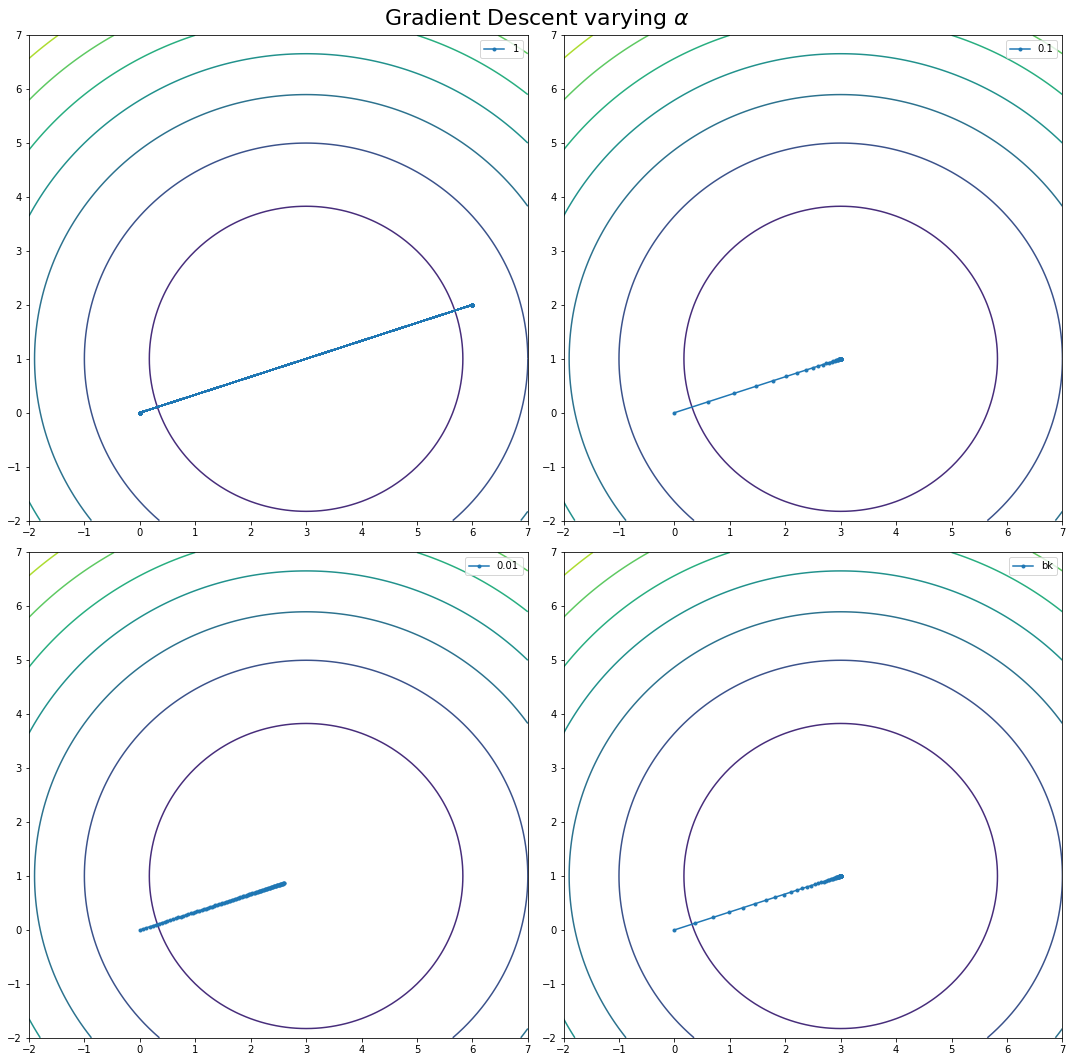
\includegraphics[width=0.8\linewidth]{1_c.png}
  \caption{Contour plot for the first function.}
  \label{fig:1c}
\end{figure}

As it can be seen, with $\alpha=1$ the minimum is never reached: indeed the algorithm keeps "jumping" from one side of the function to the other being the step length too big to approximate the optimum, as shown in \ref{fig:1c} top-left graph.
Lowering $\alpha$ allows the algorithm to reach the minimum, at a different speed (or equivalently iterations). $\alpha=0.1$ is the best value in this case and outperforms \emph{backtracking} although the latter starts exactly from the same $\alpha$ value.
This means that, after the first iteration, the backtracking mechanism change $\alpha$ to a lower value, decreasing the convergence speed.

\section{Function \#2}
Optimize function $f:\mathbb{R}^2 \rightarrow \mathbb{R}$ such that
\begin{equation}
  f(x_1,x_2)=10(x_1-1)^2+(x_2-2)^2
\end{equation}
where the true optimum is $x^*=(1,2)^T$.

The derivative of $f$ is
\begin{equation}
  \nabla f(x_1,x_2)= [20(x_1-1),2(x_2-2)]
\end{equation}

Graphs in \ref{fig:2} and \ref{fig:2c} show the value of the gradient $\nabla f(\vec{x})$ and the distance between $\vec{x}_{true}$ and $\vec{x}_k$ for each iteration and for different values of $\alpha$.
\begin{figure}[!htb]
  \minipage{0.5\textwidth}
    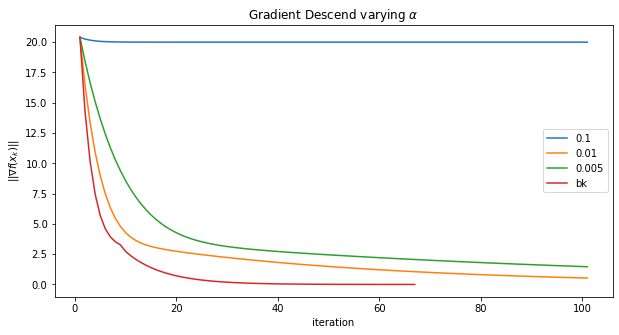
\includegraphics[width=\linewidth]{2_a.png}
  \endminipage\hfill
  \minipage{0.5\textwidth}
    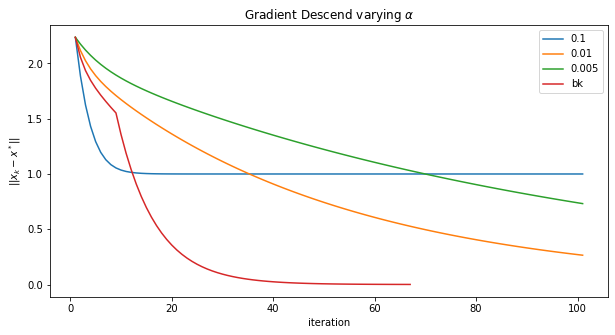
\includegraphics[width=\linewidth]{2_k.png}
  \endminipage\hfill
  \caption{Gradient Descent applied to second function.}
  \label{fig:2}
\end{figure}
\begin{figure}[!htb]
  \center
  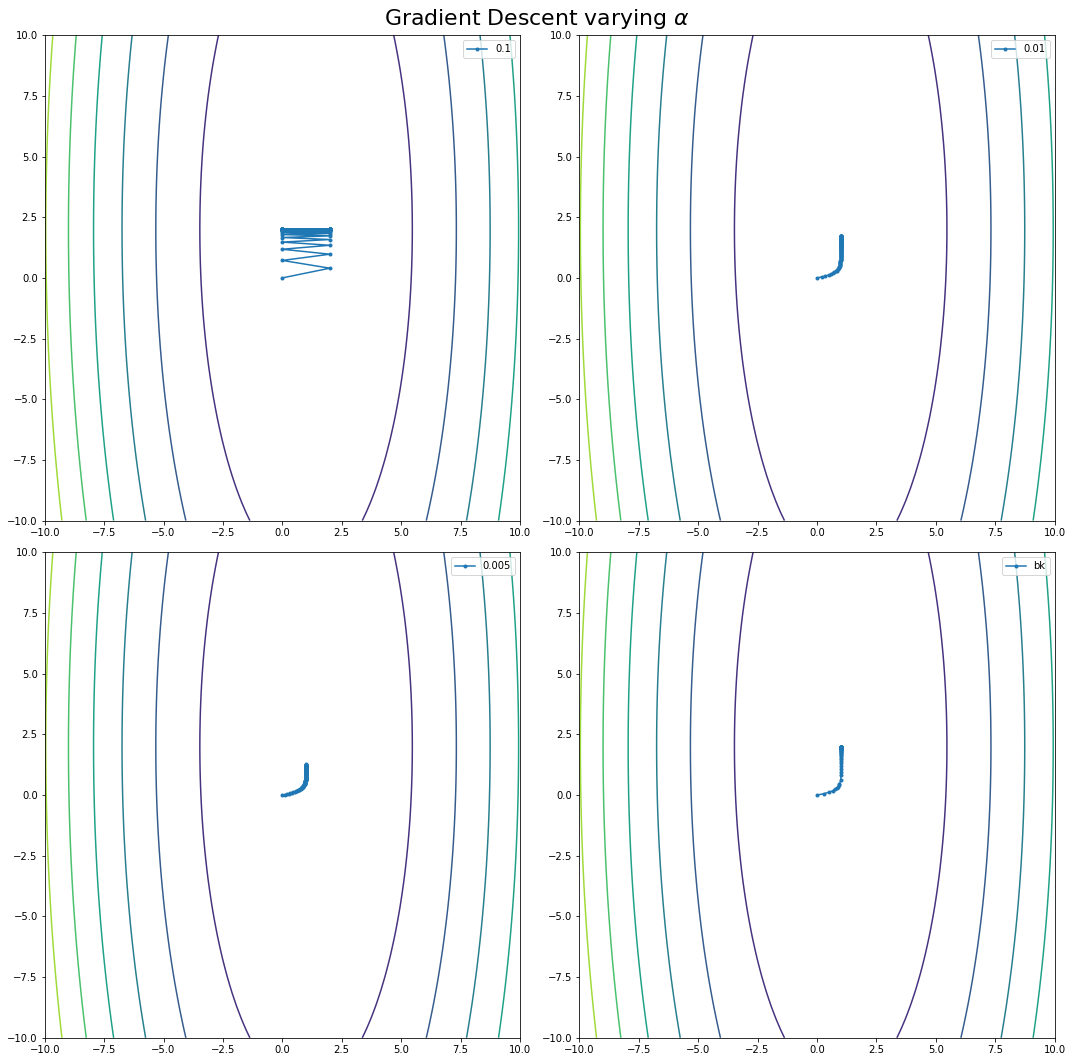
\includegraphics[width=0.8\linewidth]{2_c.png}
  \caption{Contour plot for the second function.}
  \label{fig:2c}
\end{figure}

In this case, being the function an asymmetrical paraboloid \ref{fig:2c}, GD can go closer to the minimum also with $\alpha=1$, but the optimization can not go further because for the orthogonal axe the $\alpha$ value is too big.
Here the \emph{backtracking} is faster then the $\alpha$s chosen because is able to adapt to different scale of the axes.
The visible step in the backtracking plot is the change in the $\alpha$ value and it clearly shows the speed up in convergence.

\section{Function \#3}
Optimize function $f:\mathbb{R}^2 \rightarrow \mathbb{R}$ such that
\begin{equation}
  f(x)=\frac{1}{2}||Ax-b||_2^2
\end{equation}
where $A\in \mathbb{R}^{n\times n}$ is the Vandermonde matrix  associated with the vector $\vec{v}\in\mathbb{R}^n$ that contains
n equispaced values in the interval [0; 1], and $\vec{b}\in\mathbb{R}^n$ is computed by first setting $x_{true}=\vec{1}$ and then $\vec{b} = A\vec{x}_{true}$.

As a reminder, the Vandermonde matrix V is a matrix with the terms of a geometric progression in each row, i.e. $V_{ij}=x_i^{j-1}$.

The derivative of $f$ is
\begin{equation}
  \nabla f(x)= (x^TA^T-b^T)A
\end{equation}
By definition, the Vandermonde matrix's shape depends on the chosen \emph{n}. In this exercise I have experimented with n=(5, 10, 15). Results are shown below.

Graphs in \ref{fig:3}, \ref{fig:3_n10} and \ref{fig:3_n15} show the value of the gradient $\nabla f(\vec{x})$ for each iteration and for different values of $\alpha$ and \emph{n}.

\begin{figure}[!htb]
  \center
  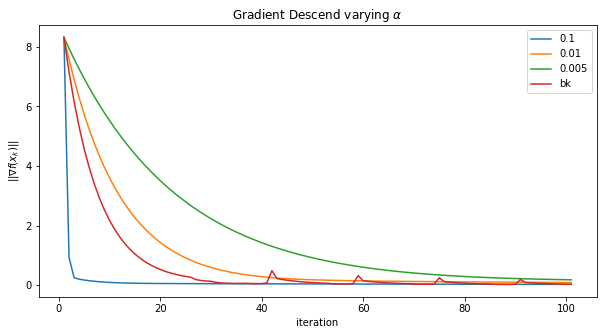
\includegraphics[width=0.8\linewidth]{3_a.png}
  \caption{Gradient Descent applied to third function with n=5.}
  \label{fig:3}
\end{figure}

\begin{figure}[!htb]
  \minipage{0.5\textwidth}
    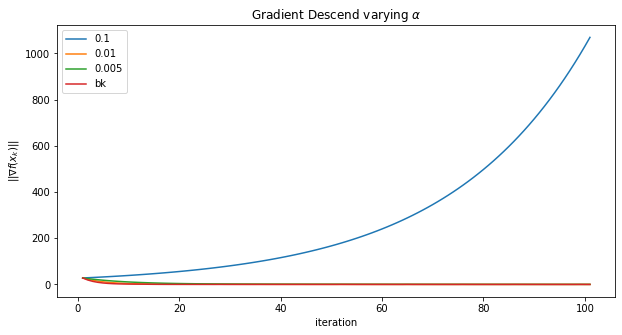
\includegraphics[width=\linewidth]{3_a_n10_1.png}
  \endminipage\hfill
  \minipage{0.5\textwidth}
    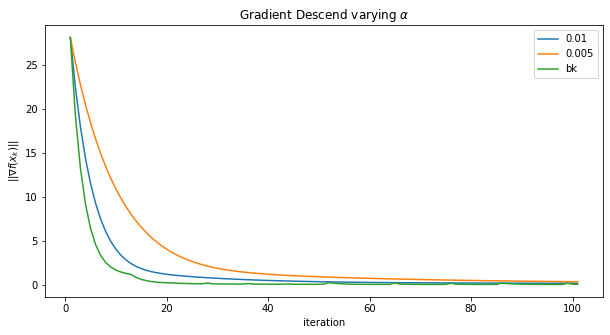
\includegraphics[width=\linewidth]{3_a_n10_2.png}
  \endminipage\hfill
  \caption{Gradient Descent applied to third function with n=10 with and without $\alpha=0.1$.}
  \label{fig:3_n10}
\end{figure}

\begin{figure}[!htb]
  \minipage{0.5\textwidth}
    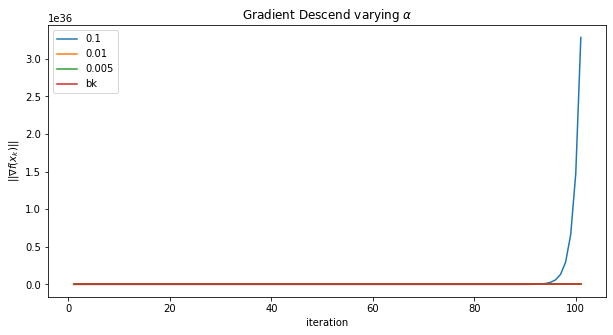
\includegraphics[width=\linewidth]{3_a_n15_1.png}
  \endminipage\hfill
  \minipage{0.5\textwidth}
    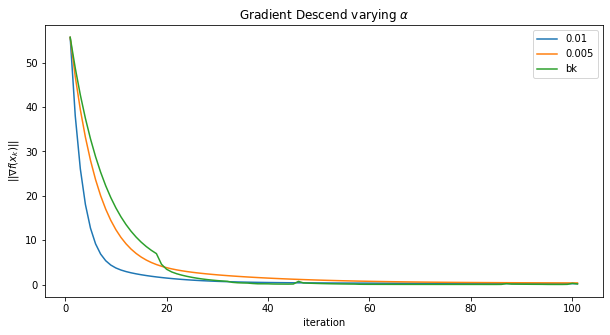
\includegraphics[width=\linewidth]{3_a_n15_2.png}
  \endminipage\hfill
  \caption{Gradient Descent applied to third function with n=15 with and without $\alpha=0.1$.}
  \label{fig:3_n15}
\end{figure}

In this case it can be seen how the function $f$ is sensitive to the combination of $\alpha$ and \emph{n}: my idea is that the Vandermonde matrix is strongly ill-conditioned, being $k\approx 686, 15*10^6$ and $403*10^9$ for respectively $n=5, 10, 15$.
For this reason, when $\alpha$ is too big, a small error in the wrong direction leads to a divergence in the approximation error.
Indeed, the Vandermonde matrix represents a linear map from the coefficient of a polinomial to its values, computed in the values of the Vandermonde matrix, so when dealing with polinomial of high grade it is easy to encounter divergent gradient if $\alpha$ is not correctly tuned.
In \ref{fig:expgd} gradient component for $A_{n=10}$ are shown.
\begin{figure}[!htb]
  \center
  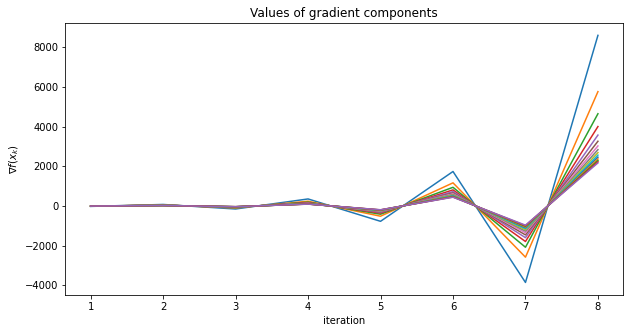
\includegraphics[width=0.8\linewidth]{exploding_gd.png}
  \caption{Gradient values for third function with n=5.}
  \label{fig:expgd}
\end{figure}

When using a smaller $\alpha$, it can be seen that the best strategy is \emph{backtracking} for n=10 and 15, because it reaches a better minimum faster, while for n=5 a fixed $\alpha=0.1$ is a good choice.
\newpage
\section{Function \#4}
Optimize function $f:\mathbb{R}^2 \rightarrow \mathbb{R}$ such that
\begin{equation}
  f(x)=\frac{1}{2}||Ax-b||_2^2 + \frac{\lambda}{2}||x||_2^2
\end{equation}

The derivative of $f$ is
\begin{equation}
  \nabla f(x)= (x^TA^T-b^T)A + \lambda x^T
\end{equation}
where A in both previous equations, is the same Vandermonde matrix with \emph{n}=5 used in the previous experiment and $\lambda\in [0,1]$ is a constant.
The function $f$ is the well known Ridge regression, a regression model employed when the independent variables are highly correlated, or in other words, the data show multi-collinearity.
The parameter $\lambda$ is the regularization parameter, also called "penalty term", and it is used in order to prevent overfitting when training a machine learning model.

Graphs \ref{fig:4}, \ref{fig:4_n10} and \ref{fig:4_n15} show the value of the gradient $\nabla f(\vec{x})$ for each iteration and for different values of $\alpha$.

\begin{figure}[!htb]
  \center
  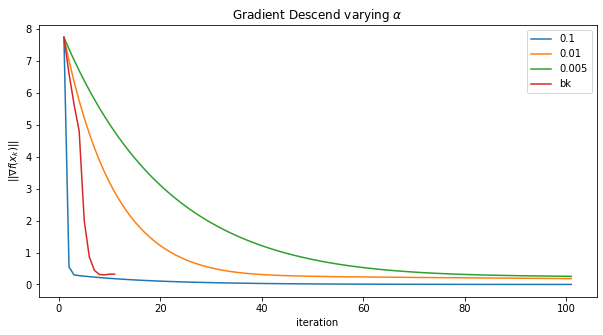
\includegraphics[width=0.8\linewidth]{4_a.png}
  \caption{Gradient Descent applied to fourth function.}
  \label{fig:4}
\end{figure}

\begin{figure}[!htb]
  \minipage{0.5\textwidth}
    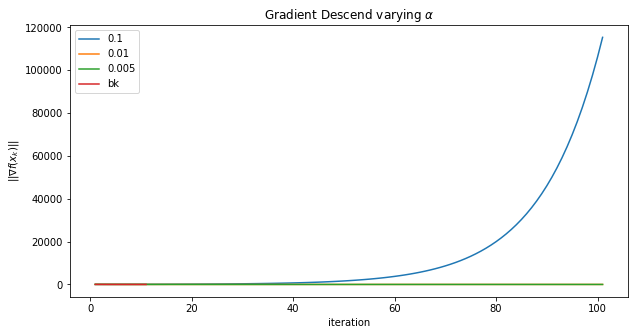
\includegraphics[width=\linewidth]{4_a_n10_1.png}
  \endminipage\hfill
  \minipage{0.5\textwidth}
    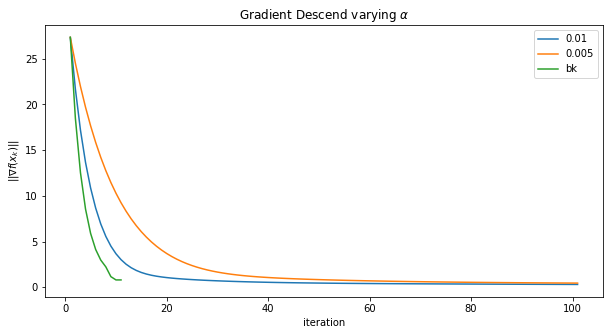
\includegraphics[width=\linewidth]{4_a_n10_2.png}
  \endminipage\hfill
  \caption{Gradient Descent applied to fourth function with n=10 with and without $\alpha=0.1$.}
  \label{fig:4_n10}
\end{figure}

\begin{figure}[!htb]
  \minipage{0.5\textwidth}
    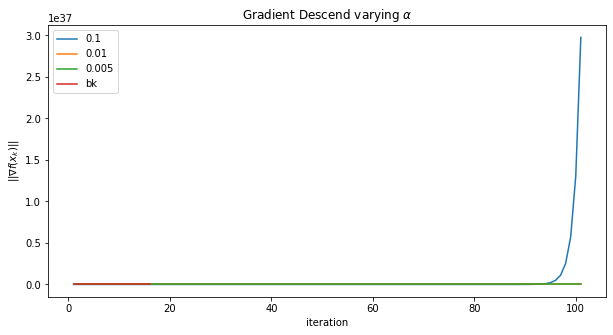
\includegraphics[width=\linewidth]{4_a_n15_1.png}
  \endminipage\hfill
  \minipage{0.5\textwidth}
    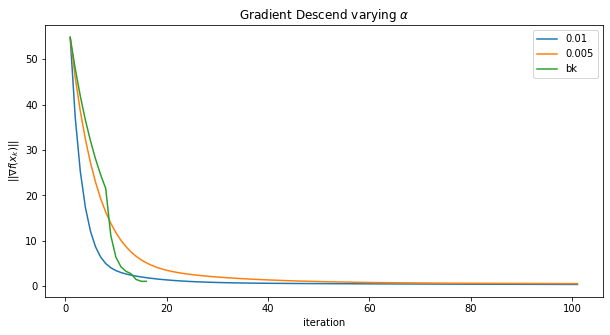
\includegraphics[width=\linewidth]{4_a_n15_2.png}
  \endminipage\hfill
  \caption{Gradient Descent applied to fourth function with n=15 with and without $\alpha=0.1$.}
  \label{fig:4_n15}
\end{figure}

\begin{figure}[!htb]
  \minipage{0.5\textwidth}
    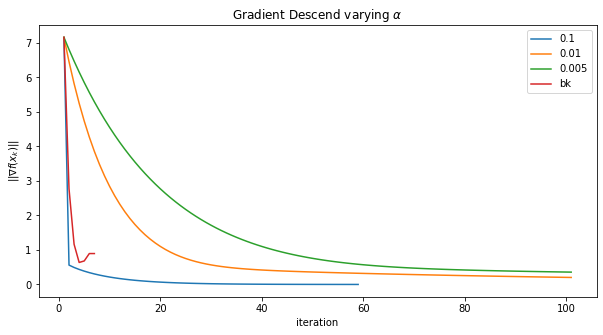
\includegraphics[width=\linewidth]{4_a_l1.png}
  \endminipage\hfill
  \minipage{0.5\textwidth}
    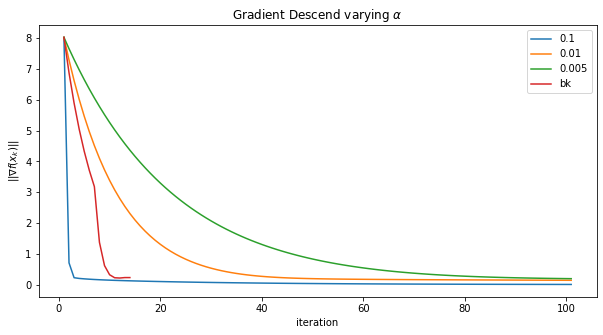
\includegraphics[width=\linewidth]{4_a_l025.png}
  \endminipage\hfill
  \caption{Gradient Descent applied to fourth function with n=5 $\lambda=1$ and $\lambda=0.25$.}
  \label{fig:4_l}
\end{figure}

Here again ita can be seen how the ill-conditioning of the Vandermonde matrix is worse than before due to the penalty term.
By removing $\alpha=0.1$ it can be seen that the best strategy is \emph{backtracking} again: indeed it reaches the best minimum faster and stops the algorithm thanks to the reaching of the convergence condition in \ref{eq:convergence}.

In \ref{fig:4_l} it can be seen how the GD behaves varying $\lambda$. In particular, it can be seen that a value of $\lambda$ close to one, prevents the algorithm from reaching a better minimum, that is instead reached when $\lambda=0.25$.
The case where $\lambda=0$ is the same as function 3.

\chapter{Exercise 2 - Stochastic Gradient Descent}\label{chap:sgd}
In the second exercise it is required to apply Stochastic Gradient Descent to a randomly generated dataset in order to simulate what is usually done in machine learning.
This time optimization is carried out in the space of weights instead of the space of \emph{x}: dataset samples are only used to evaluate the gradient while the derivatives are computed with respect the weights vector.

I chose to generate a dataset of $N=1000$ samples and as space dimension for weights vector $\vec{w} \in \mathbb{R}^{10}$.

I have run two experiment with SGD: in the first I have fixed the batch size to 100 and number of epochs to 50, run SGD on diferent values of $\alpha$ and selected the one that made the algorithm to reach the minimum faster (results in \ref{fig:sgd_a});
then I have used the $\alpha$ just found and run SGD for 20 epochs, each time with a diferent batch size from the list \emph{[1,50,100,250,500]}.
Results are shown in \ref{fig:sgd_n}.

\begin{figure}[!htb]
  \center
  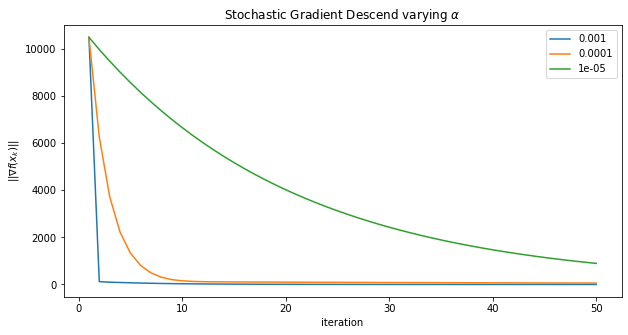
\includegraphics[width=0.8\linewidth]{sgd_a.png}
  \caption{SGD varying $\alpha$.}
  \label{fig:sgd_a}
\end{figure}

\begin{figure}[!htb]
  \center
  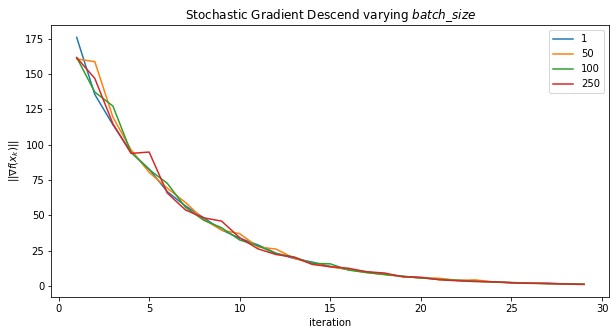
\includegraphics[width=0.8\linewidth]{sgd_n.png}
  \caption{SGD with $\alpha=1e-3$ varying \emph{batch_size} parameter.}
  \label{fig:sgd_n}
\end{figure}



Here it can be observed that the relation between convergence speed and $\alpha$ value is monotonic: indeed the biggest $\alpha$ (among the chosen ones) allows SGD to reach the minimum faster, and when decreasing $\alpha$ convergence speed slows down.
I tried also using $\alpha=0.01$ but after around 20 iterations the algorithm diverged, so I removed it from the graph.

Then I have taken the best $\alpha$ and experimented with the batch size. In general there is no a one direction path in choosing first $\alpha$ and then $batch\_size$, actually also this choice should be optimized by alternatively changing the two parameters until the best configuration is found.

In this case it can be observed that a different batch size can make the learning phase slower and noisier. For example, just look at the red line and the blue one in \ref{fig:sgd_n}.
The reason is that more smaller updates are better than one single big update: indeed the algorithm performs $|\mathbb{D}|/batch\_size$ updates at each epoch, so the smaller the batch size the greater the number of updates and so the convergence speed.
The drawback is obviously the computation burden, being the mini batch size more resource demanding.

\chapter{Conclusion}\label{chap:conclusion}
In this exercise we experimented around Gradient Descent and Stochastic Gradient Descent techniques. We saw how they are effective in optimizing almost any kind of ("optimizable") function.
In case of convex oprimization, GD and SGD always reach the global optimum, while in case of non-convex function it depends on the starting point and in general it is not certain that it will reach a global minimum. A caveat that is worth to highlight here is that convergence of GD or SGD does not mean having reached the best minimum, because there would be no way to distinuish between a local and a global one.

From a machine learning point of view, we saw that is crucial to find the right configuration of hyperparameters, indeed also the best model (from a mathematical point of view) could fail to reach convergence due to a misconfiguration of hyperparameters.
For this reason, a crucial step in machine learning is the validation phase, where the algorithm hyperparameter are fine-tuned on a never seen dataset partition.

In this exercise there would be a huge number of combination of hyperparameters to play with and test, so I decided to restrict the range to the value reported in this work.

\end{document}
